\chapter{Le memorie}
La memoria \`e fondamentale per il funzionamento di un compilatore. \`E necessario poterci leggere e scrivere dati. La memoria indirizzata direttamente (memoria 
principale o cache) \`e volatile ed \`e limitata dallo spazio di indirizzamento dal compilatore. Esiste una memoria indirizzata indirettamente o periferica, permanente
con uno spazio di indirizzamento software non limitato dal processore. Le informazioni sulla memoria principale sono disponibili al processore in qualsiasi momento, 
mentre le informazioni nella memoria periferica devono essere prima trasferite a quella principale. Questo trasferimento \`e tipicamente mediato dal sistema operativo.
\begin{itemize}
\item Si intende per tempo di accesso il tempo di un'operazione di lettura o scrittura nella memoria.
\item Il tempo di ciclo \`e il tempo che intercorre tra l'inizio di due operazioni tra locazioni diverse.
\item Accesso casuale: non vi \`e alcuna relazione o ordine tra i dati salvati, tipico delle memorie a semiconduttori.
\item Accesso sequenziale: l'accesso alla memoria \`e ordinato o semi ordinato, il tempo di accesso dipende dalla posizione, tipico dei dischi o dei nastri.
\item RAM (random access memory) memoria scrivibile leggibile a semiconduttori, con tempo di accesso indipendente dalla posizione del dato.
\item ROM (read only memory) memoria a semiconduttori in sola lettura pu\`o avere accesso casuale o sequenziale. 
\end{itemize}
\section{Memorie RAM a semiconduttori}
Queste memorie memorizzano singoli bit spesso organizzati in byte e o word. Data una capacit\`a N la memoria pu\`o essere organizzata in diversi modi a seconda del
parallelismo, influenzando il numero di pin I/O necessari al circuito integrato che la implementa.
\subsection{Memorie statiche SRAM}
Sono memorie in cui i bit possono essere salvati indefinitamente fintanto che rimangono alimentate, sono estremamente veloci e consumano poca corrente, ma sono care
in quanto richiedono molte componenti per ciascuna cella di memorizzazione.
\begin{figure}
  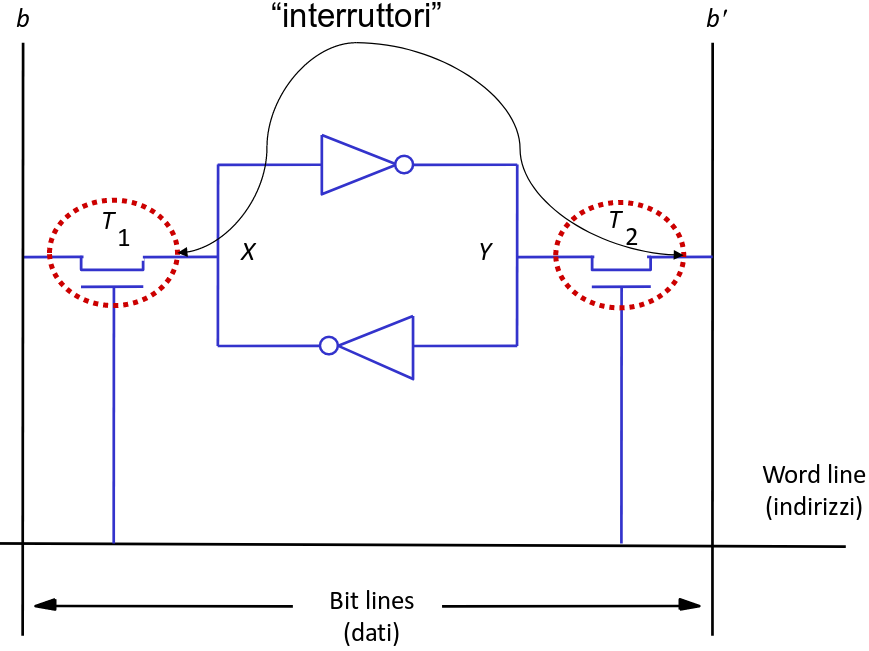
\includegraphics[scale=0.2]{Pictures/SRAM.png}
  \caption{Un bit in SRAM}
  \label{fig:boat1}
\end{figure}
Si consideri che $b=NOT(b')$, i circuiti di terminazione della linea di bit (sense/write circuit) interfacciano il mondo esterno che non accede mai direttamente alle 
celle, la loro presenza contemporanea riduce gli errori. In caso di scrittura la linea di word \`e alta e chiude $T_1$ e $T_2$, il valore presente su b e b', linee di 
pilotaggio viene salvato nel latch a doppio NOT. In caso di lettura la linea di word \`e alta e chiude $T_1$ e $T_2$, il le linee b e b' sono tenute in stato di alta 
impedenza e il valore in X e Y viene copiato in b e b'. Se la linea di word \`e bassa il consumo \`e nullo. 
\subsection{Memorie DRAM}
Sono le memorie pi\`u diffuse in quanto economiche e a densit\`a elevata, in quanto la memoria viene ottenuta sotto forma di carica di un condensatore. Hanno bisogno
per\`o di un costante refresh altrimenti la carica si disperderebbe a causa di correnti parassite.
\begin{figure}
  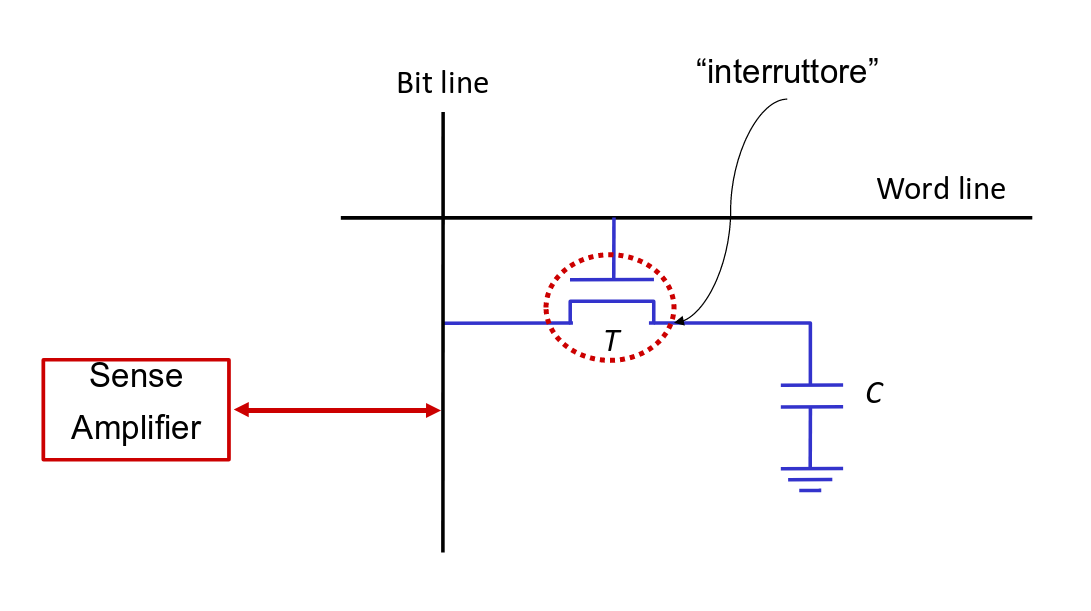
\includegraphics[scale=0.2]{Pictures/DRAM.png}
  \caption{Un bit in DRAM}
  \label{fig:boat1}
\end{figure}
In caso di operazione di scrittura la linea di word \`e alta e chiude T e il valore di b viene copiato su C. In caso di lettura la linea di word chiude T e si utilizza
un apposito circuito che se la tensione di C \`e sopra una certa soglia pilota la linea b alla tensione di alimentazione ricaricando C, altrimenti mette b a terra 
scaricando C.
\subsubsection{Refresh}
Nel momento in cui T \`e aperto il condensatore comincia a caricarsi o scaricarsi a causa di correnti parassite sul semiconduttore e si rende necessario quindi 
periodcamente rinfrescare i dati attraverso un'operazione di lettura. In genere la memoria contiene un circuito per la lettura periodica della memoria, pertanto 
l'utente non se ne deve preoccupare.
\subsubsection{Multiplazione degli indirizzi}
Data l'elevata integrazione delle DRAM il numero di pin I/O diventa un problema, pertanto \`e usuale multiplare nel tempo l'indirizzo delle righe e delle colonne negli
stessi fili. Le memorie non sono indirizzabili al bit, per cui righe e colonne si riferiscono a byte e non a bit. 
\subsubsection{Modo di accesso veloce}
L'accesso ai dati della memoria DRAM avviene da blocchi o pagine di memoria: l'indirizzo viene separato in row address selector e column address selector, il primo dei 
quali estrae una riga dalla pagina e il secondo la colonna dalla riga. \`E possibile, attraverso il fast page mode (FPM) evitare di riselezionare la riga ad ogni accesso
se le posizioni sono consecutive con aumenti delle prestazioni significativi. 
\subsection{Memorie DRAM sincrone SDRAM}
Le DRAM viste prima sono dette asincrone in quanto non esiste una precisa temporizzazione di accesso, ma la dinamica viene governata dai RAS e dai CAS. Il processore
deve tenerne conto in quanto pu\`o generare problemi in fase di refresh. Aggiungendo dei buffer di memorizzazione degli ingressi e delle uscite si pu\`o ottenere 
un funzionamento sincrono disaccoppiando lettura e scrittura dal refresh, ottenendo automaticamente un FPM pilotato dal clock. 
\subsection{Double data rate SDRAM: DDR-SDRAM}
Una SDRAM che consente il trasferimento dei file sia sul fronte positivo che quello negativo del clock. Latenza uguale a una DRAM normale ma banda doppia, le memorie
sono separate in due banchi uno per le locazioni pari sul fronte positivo e l'altro per le locazioni dispari sul fronte negativo. Le locazioni contigue sono in banchi
separati pertanto si pu\`o fare un accesso interlacciato. 
\section{Velocit\`a e prestazione}
\subsubsection{Latenza}
Il tempo di accesso ad una singola parola, d\`a un indicazione al tempo che un processore dovr\`a aspettare un dato dalla memoria nel caso peggiore.
\subsubsection{Velocit\`a o banda}
Indica la velocit\`a di trasferimento massima in FPM, importante per operazioni in FPM che sono legate all'uso di memorie cache interne ai processori. 
\section{Gerarchie di memoria}
Si pu\`o ottimizzare l'utilizzo di memorie in modo da dare l'impressione di avere una grande memoria veloce.
\subsubsection{Localit\`a temporale}
Quando si fa uso di una locazione \`e molto probabile che verr\`a riutilizzata presto.
\subsubsection{Localit\`a spaziale}
Quando si fa riferimento ad una locazione \`e molto probabile che nelle operazioni successive si far\`a riferimento alle locazioni successive.
\subsection{Struttura della gerarchia}
Costi e velocit\`a delle memorie creano una propensione a utilizzare delle piccole e veloci vicino al processore che si ingrandiscono e rallentano allontanandosi da 
esso.
\subsubsection{Terminologia}
\begin{itemize}
\item Si indica con blocco l'unit\`a minima di informazione che pu\`o essere presente o assente in un livello.
\item Hit rate: la frequenza di accesso, la frazione degli accessi in cui trovo il blocco nel livello superiore. 
\item Miss rate: il complementare dell'hit rate.
\item Tempo di hit: il tempo che occorre per trovare il dato quando lo trovo nel livello superiore. 
\item Penalit\`a di miss: il tempo necessario per accedere al dato se non lo trovo nel livello superiore
\end{itemize}
La penalit\`a di miss \`e molto maggiore del tempo di hit e del trasferimento in memoria di un singolo dato, pertanto \`e cruciale che non avvenga troppo spesso. 
\subsection{Cache}
Un posto sicuro, o nascosto dove riporre i dati, nascosto in quanto \`e impossibile accedervi direttamente. Per capire se un dato \`e nella cache o no si pu\`o 
utilizzare una cache a mappatura diretta, ovvero a ogni indirizzo della memoria corrisponde una precisa locazione della cache, l'indirizzo di locazione dove un indirizzo
\`e mappato \`e l'indirizzo del blocco modulo numero di blocchi nella cache. Se il numero di elementi della cache \`e a potenza di due \`e sufficiente prendere i bit 
meno significativi dell'indirizzo in numero pari al logaritmo in base due della potenza della cache. Siccome molte parole possono essere mappate sullo stesso blocco di 
cache per capire se in un dato momento vi si trova l'indirizzo ricercato si ricorre ad un campo, detto tag, che contiene informazione sufficiente a risalire al blocco 
correntemente salvato in memoria, si possono utilizzare per esempio i bit pi\`u significativi di una parola per trovare la locazione in cache dove l'indirizzo \`e 
mappato. Vengono utilizzati i bit pi\`u significativi per capire se nel blocco di cache viene memorizzato l'elemento richiesto, inoltre c'\`e un blocco di validit\`a
che dice se quello che viene memorizzato in un blocco di cache in un dato momento \`e quello richiesto. 
\subsubsection{Prestazioni}
Blocchi di cache molto grande esaltano la localit\`a spaziale e diminuiscono la probabilit\`a di miss. Tuttavia a parit\`a di grandezza della cache blocchi molto grandi 
diminuisce l'efficacia della localit\`a temporale, oltre a generare dei miss con costo elevato. Si necessita pertanto di dover trovare un equilibrio. 
\subsubsection{Gestione delle miss}
La presenza di una cache modifica la gestione della pipeline solo nel caso in cui ci sono delle miss, quando bisogna generare uno stallo nella pipeline per gestire il
trasferimento da memoria principale a cache. Per una miss sulla memoria istruzioni bisogner\`a inviare alla memoria il valora PC-4, eseguire una lettura, scriverne il
risultato aggiornando il tag e far ripartire la fetch. Gli accessi in lettura alla memoria dati avvengono alla stessa maniera.
\subsubsection{Miss in scrittura}
Gli accessi in scrittura sono delicati in quanto possono generare delle inconsistenze. Possono venire implementate due politiche:
\begin{enumerate}
\item Write-through, in cui ogni scrittura viene fatta direttamente in memoria principale, eliminando i problemi di consistenza ma aumentando i costi, si pu\`o impiegare
un buffer di scrittura, una coda con tutte le scritture in attesa di essere completate.
\item Write-back, in cui se il blocco \`e in cache le scritture avvengono localmente in cache e l'update viene fatto solo quando il blocco viene rimpiazzato. Conveniente
in presenza di numerose scritture. 
\end{enumerate}
\subsubsection{Cache completamente associativa}
In questo tipo di cache si pu\`o mappare qualsiasi tipo di blocco in qualsiasi blocco di cache, il loro problema \`e che rendono necesario cercare ovunque il dato, per
essere efficiente su tutti i blocchi in parallelo, si necessitano pertanto n comparatori che operino su n blocchi. Il costo \`e molto elevato, pertanto viene utilizzata 
solo per cache molto piccole. 
\subsubsection{Cache set-associativa}
\`E una via di mezzo tra la mappatura diretta e la completamente associativa: ogni blocco di memoria pu\`o essere mappato su una linea di n blocchi diversi di cache. Si combinano pertanto le due idee: a 
ciascun blocco di memoria viene associata una certa linea, pertanto uno degli n blocchi di quella liena su cui si pu\`o mappare il blocco di memoria e all'interno della linea si effettua una ricerca parallela come
se fosse una cache completamente associativa.  Ovvero un blocco di memoria viene mappato nella linea data da indirizzo blocco modulo numero linee della cache. Pertanto per trovare il blocco all'interno della
linea si deve confrontare in parallelo il tag del blocco con tuti i tag dei blocchi di quella linea.  Aumentando l'associativit\`a diminuisce la frequenza di miss, ma si rendono necessarie operazioni complesse. 
Inoltre nelle cache a mappatura diretta in caso di miss so sicuramente chi sostituire, nelle cache associative si possono utilizzare diverse strategie, come una FIFO o una Least Recently Used.
